\section{Spark::Sp\-Stream\-Basis Class Reference}
\label{classSpark_1_1SpStreamBasis}\index{Spark::SpStreamBasis@{Spark::SpStreamBasis}}
{\tt \#include $<$Sp\-Stream\-Basis.h$>$}

Inheritance diagram for Spark::Sp\-Stream\-Basis:\begin{figure}[H]
\begin{center}
\leavevmode
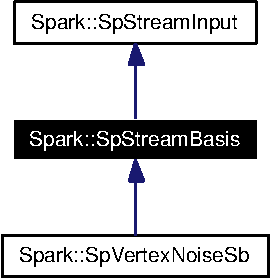
\includegraphics[width=82pt]{classSpark_1_1SpStreamBasis__inherit__graph}
\end{center}
\end{figure}
Collaboration diagram for Spark::Sp\-Stream\-Basis:\begin{figure}[H]
\begin{center}
\leavevmode
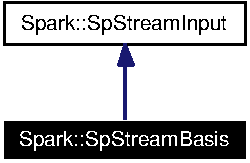
\includegraphics[width=77pt]{classSpark_1_1SpStreamBasis__coll__graph}
\end{center}
\end{figure}


\subsection{Detailed Description}
Abstract base class for a stream basis for spectral synthesis. 

Definition at line 32 of file Sp\-Stream\-Basis.h.\subsection*{Public Member Functions}
\begin{CompactItemize}
\item 
{\bf Sp\-Stream\-Basis} ()
\begin{CompactList}\small\item\em Construction:. \item\end{CompactList}\item 
virtual {\bf $\sim$Sp\-Stream\-Basis} ()
\item 
virtual bool {\bf has\-Changed} ()=0
\begin{CompactList}\small\item\em Methods:. \item\end{CompactList}\item 
virtual bool {\bf send\-Output\-To\-Buffer} ({\bf Sp\-Stream\-Buffer} $\ast$pk\-Buffer, {\bf Sp\-Stream\-Feedback} $\ast$pk\-Copy)=0
\item 
virtual void {\bf set\-Weight} (float f\-X)
\item 
virtual float {\bf get\-Weight} ()
\item 
virtual void {\bf set\-Offset} (float, float, float)
\item 
virtual void {\bf get\-Offset} (float \&, float \&, float \&) const
\item 
virtual void {\bf set\-Scale} (float, float, float)
\item 
virtual void {\bf get\-Scale} (float \&, float \&, float \&) const
\end{CompactItemize}


\subsection{Constructor \& Destructor Documentation}
\index{Spark::SpStreamBasis@{Spark::Sp\-Stream\-Basis}!SpStreamBasis@{SpStreamBasis}}
\index{SpStreamBasis@{SpStreamBasis}!Spark::SpStreamBasis@{Spark::Sp\-Stream\-Basis}}
\subsubsection{\setlength{\rightskip}{0pt plus 5cm}Spark::Sp\-Stream\-Basis::Sp\-Stream\-Basis ()\hspace{0.3cm}{\tt  [inline]}}\label{classSpark_1_1SpStreamBasis_a0}


Construction:. 

Definition at line 38 of file Sp\-Stream\-Basis.h.\index{Spark::SpStreamBasis@{Spark::Sp\-Stream\-Basis}!~SpStreamBasis@{$\sim$SpStreamBasis}}
\index{~SpStreamBasis@{$\sim$SpStreamBasis}!Spark::SpStreamBasis@{Spark::Sp\-Stream\-Basis}}
\subsubsection{\setlength{\rightskip}{0pt plus 5cm}virtual Spark::Sp\-Stream\-Basis::$\sim${\bf Sp\-Stream\-Basis} ()\hspace{0.3cm}{\tt  [inline, virtual]}}\label{classSpark_1_1SpStreamBasis_a1}


Definition at line 43 of file Sp\-Stream\-Basis.h.

\subsection{Member Function Documentation}
\index{Spark::SpStreamBasis@{Spark::Sp\-Stream\-Basis}!getOffset@{getOffset}}
\index{getOffset@{getOffset}!Spark::SpStreamBasis@{Spark::Sp\-Stream\-Basis}}
\subsubsection{\setlength{\rightskip}{0pt plus 5cm}virtual void Spark::Sp\-Stream\-Basis::get\-Offset (float \&, float \&, float \&) const\hspace{0.3cm}{\tt  [inline, virtual]}}\label{classSpark_1_1SpStreamBasis_a7}




Reimplemented in {\bf Spark::Sp\-Vertex\-Noise\-Sb} {\rm (p.\,\pageref{classSpark_1_1SpVertexNoiseSb_a10})}.

Definition at line 72 of file Sp\-Stream\-Basis.h.\index{Spark::SpStreamBasis@{Spark::Sp\-Stream\-Basis}!getScale@{getScale}}
\index{getScale@{getScale}!Spark::SpStreamBasis@{Spark::Sp\-Stream\-Basis}}
\subsubsection{\setlength{\rightskip}{0pt plus 5cm}virtual void Spark::Sp\-Stream\-Basis::get\-Scale (float \&, float \&, float \&) const\hspace{0.3cm}{\tt  [inline, virtual]}}\label{classSpark_1_1SpStreamBasis_a9}




Reimplemented in {\bf Spark::Sp\-Vertex\-Noise\-Sb} {\rm (p.\,\pageref{classSpark_1_1SpVertexNoiseSb_a8})}.

Definition at line 82 of file Sp\-Stream\-Basis.h.\index{Spark::SpStreamBasis@{Spark::Sp\-Stream\-Basis}!getWeight@{getWeight}}
\index{getWeight@{getWeight}!Spark::SpStreamBasis@{Spark::Sp\-Stream\-Basis}}
\subsubsection{\setlength{\rightskip}{0pt plus 5cm}virtual float Spark::Sp\-Stream\-Basis::get\-Weight ()\hspace{0.3cm}{\tt  [inline, virtual]}}\label{classSpark_1_1SpStreamBasis_a5}


Definition at line 62 of file Sp\-Stream\-Basis.h.\index{Spark::SpStreamBasis@{Spark::Sp\-Stream\-Basis}!hasChanged@{hasChanged}}
\index{hasChanged@{hasChanged}!Spark::SpStreamBasis@{Spark::Sp\-Stream\-Basis}}
\subsubsection{\setlength{\rightskip}{0pt plus 5cm}virtual bool Spark::Sp\-Stream\-Basis::has\-Changed ()\hspace{0.3cm}{\tt  [pure virtual]}}\label{classSpark_1_1SpStreamBasis_a2}


Methods:. 



Implements {\bf Spark::Sp\-Stream\-Input} {\rm (p.\,\pageref{classSpark_1_1SpStreamInput_a2})}.



Implemented in {\bf Spark::Sp\-Vertex\-Noise\-Sb} {\rm (p.\,\pageref{classSpark_1_1SpVertexNoiseSb_a15})}.

\index{Spark::SpStreamBasis@{Spark::Sp\-Stream\-Basis}!sendOutputToBuffer@{sendOutputToBuffer}}
\index{sendOutputToBuffer@{sendOutputToBuffer}!Spark::SpStreamBasis@{Spark::Sp\-Stream\-Basis}}
\subsubsection{\setlength{\rightskip}{0pt plus 5cm}virtual bool Spark::Sp\-Stream\-Basis::send\-Output\-To\-Buffer ({\bf Sp\-Stream\-Buffer} $\ast$ {\em pk\-Buffer}, {\bf Sp\-Stream\-Feedback} $\ast$ {\em pk\-Copy})\hspace{0.3cm}{\tt  [pure virtual]}}\label{classSpark_1_1SpStreamBasis_a3}




Implements {\bf Spark::Sp\-Stream\-Input} {\rm (p.\,\pageref{classSpark_1_1SpStreamInput_a3})}.

\index{Spark::SpStreamBasis@{Spark::Sp\-Stream\-Basis}!setOffset@{setOffset}}
\index{setOffset@{setOffset}!Spark::SpStreamBasis@{Spark::Sp\-Stream\-Basis}}
\subsubsection{\setlength{\rightskip}{0pt plus 5cm}virtual void Spark::Sp\-Stream\-Basis::set\-Offset (float, float, float)\hspace{0.3cm}{\tt  [inline, virtual]}}\label{classSpark_1_1SpStreamBasis_a6}




Reimplemented in {\bf Spark::Sp\-Vertex\-Noise\-Sb} {\rm (p.\,\pageref{classSpark_1_1SpVertexNoiseSb_a9})}.

Definition at line 67 of file Sp\-Stream\-Basis.h.

Referenced by Spark::Sp\-Turbulence\-Op::setup\-State().\index{Spark::SpStreamBasis@{Spark::Sp\-Stream\-Basis}!setScale@{setScale}}
\index{setScale@{setScale}!Spark::SpStreamBasis@{Spark::Sp\-Stream\-Basis}}
\subsubsection{\setlength{\rightskip}{0pt plus 5cm}virtual void Spark::Sp\-Stream\-Basis::set\-Scale (float, float, float)\hspace{0.3cm}{\tt  [inline, virtual]}}\label{classSpark_1_1SpStreamBasis_a8}




Reimplemented in {\bf Spark::Sp\-Vertex\-Noise\-Sb} {\rm (p.\,\pageref{classSpark_1_1SpVertexNoiseSb_a7})}.

Definition at line 77 of file Sp\-Stream\-Basis.h.\index{Spark::SpStreamBasis@{Spark::Sp\-Stream\-Basis}!setWeight@{setWeight}}
\index{setWeight@{setWeight}!Spark::SpStreamBasis@{Spark::Sp\-Stream\-Basis}}
\subsubsection{\setlength{\rightskip}{0pt plus 5cm}virtual void Spark::Sp\-Stream\-Basis::set\-Weight (float {\em f\-X})\hspace{0.3cm}{\tt  [inline, virtual]}}\label{classSpark_1_1SpStreamBasis_a4}




Reimplemented in {\bf Spark::Sp\-Vertex\-Noise\-Sb} {\rm (p.\,\pageref{classSpark_1_1SpVertexNoiseSb_a11})}.

Definition at line 57 of file Sp\-Stream\-Basis.h.

Referenced by Spark::Sp\-Turbulence\-Op::setup\-State().

The documentation for this class was generated from the following file:\begin{CompactItemize}
\item 
{\bf Sp\-Stream\-Basis.h}\end{CompactItemize}
